\documentclass{beamer}

\usepackage[english]{babel}
\usepackage[utf8x]{inputenc}			
\usepackage{listings}
\usepackage{xcolor}

\lstset{
    language=R,
    basicstyle=\ttfamily\small,
    backgroundcolor=\color{gray!10},
    frame=single,
    breaklines=true,
    showstringspaces=false,
    keywordstyle=\color{blue},
    commentstyle=\color{green!50!black},
    stringstyle=\color{red},
    numbers=none,
    xleftmargin=10pt,
    xrightmargin=10pt,
    framexleftmargin=5pt,
    framexrightmargin=5pt
}

\mode<presentation>						
{
  \usetheme{default}					
  \usecolortheme{default} 			
  \usefonttheme{default}  				
  \setbeamertemplate{caption}[numbered]	
}

\usepackage{graphicx}
\graphicspath{{figure/}}				% Shared figure folder for all labs
\usepackage{booktabs}
\usepackage{hyperref}					
\usepackage{subcaption}  
\usepackage{multicol}
\usepackage{hyperref}

\title{Visualization of Data}	
\author{Rex Shao-Yu Wang}								
\institute{Department of Agronomy, National Taiwan University}				
\date{March 23, 2026}								

\begin{document}

% Title page
\begin{frame}
  \titlepage
\end{frame}

% Outline
\begin{frame}{Outline}
  \tableofcontents
\end{frame}

\section{Types of Data}
\begin{frame}{Types of Data}
    \begin{figure}
        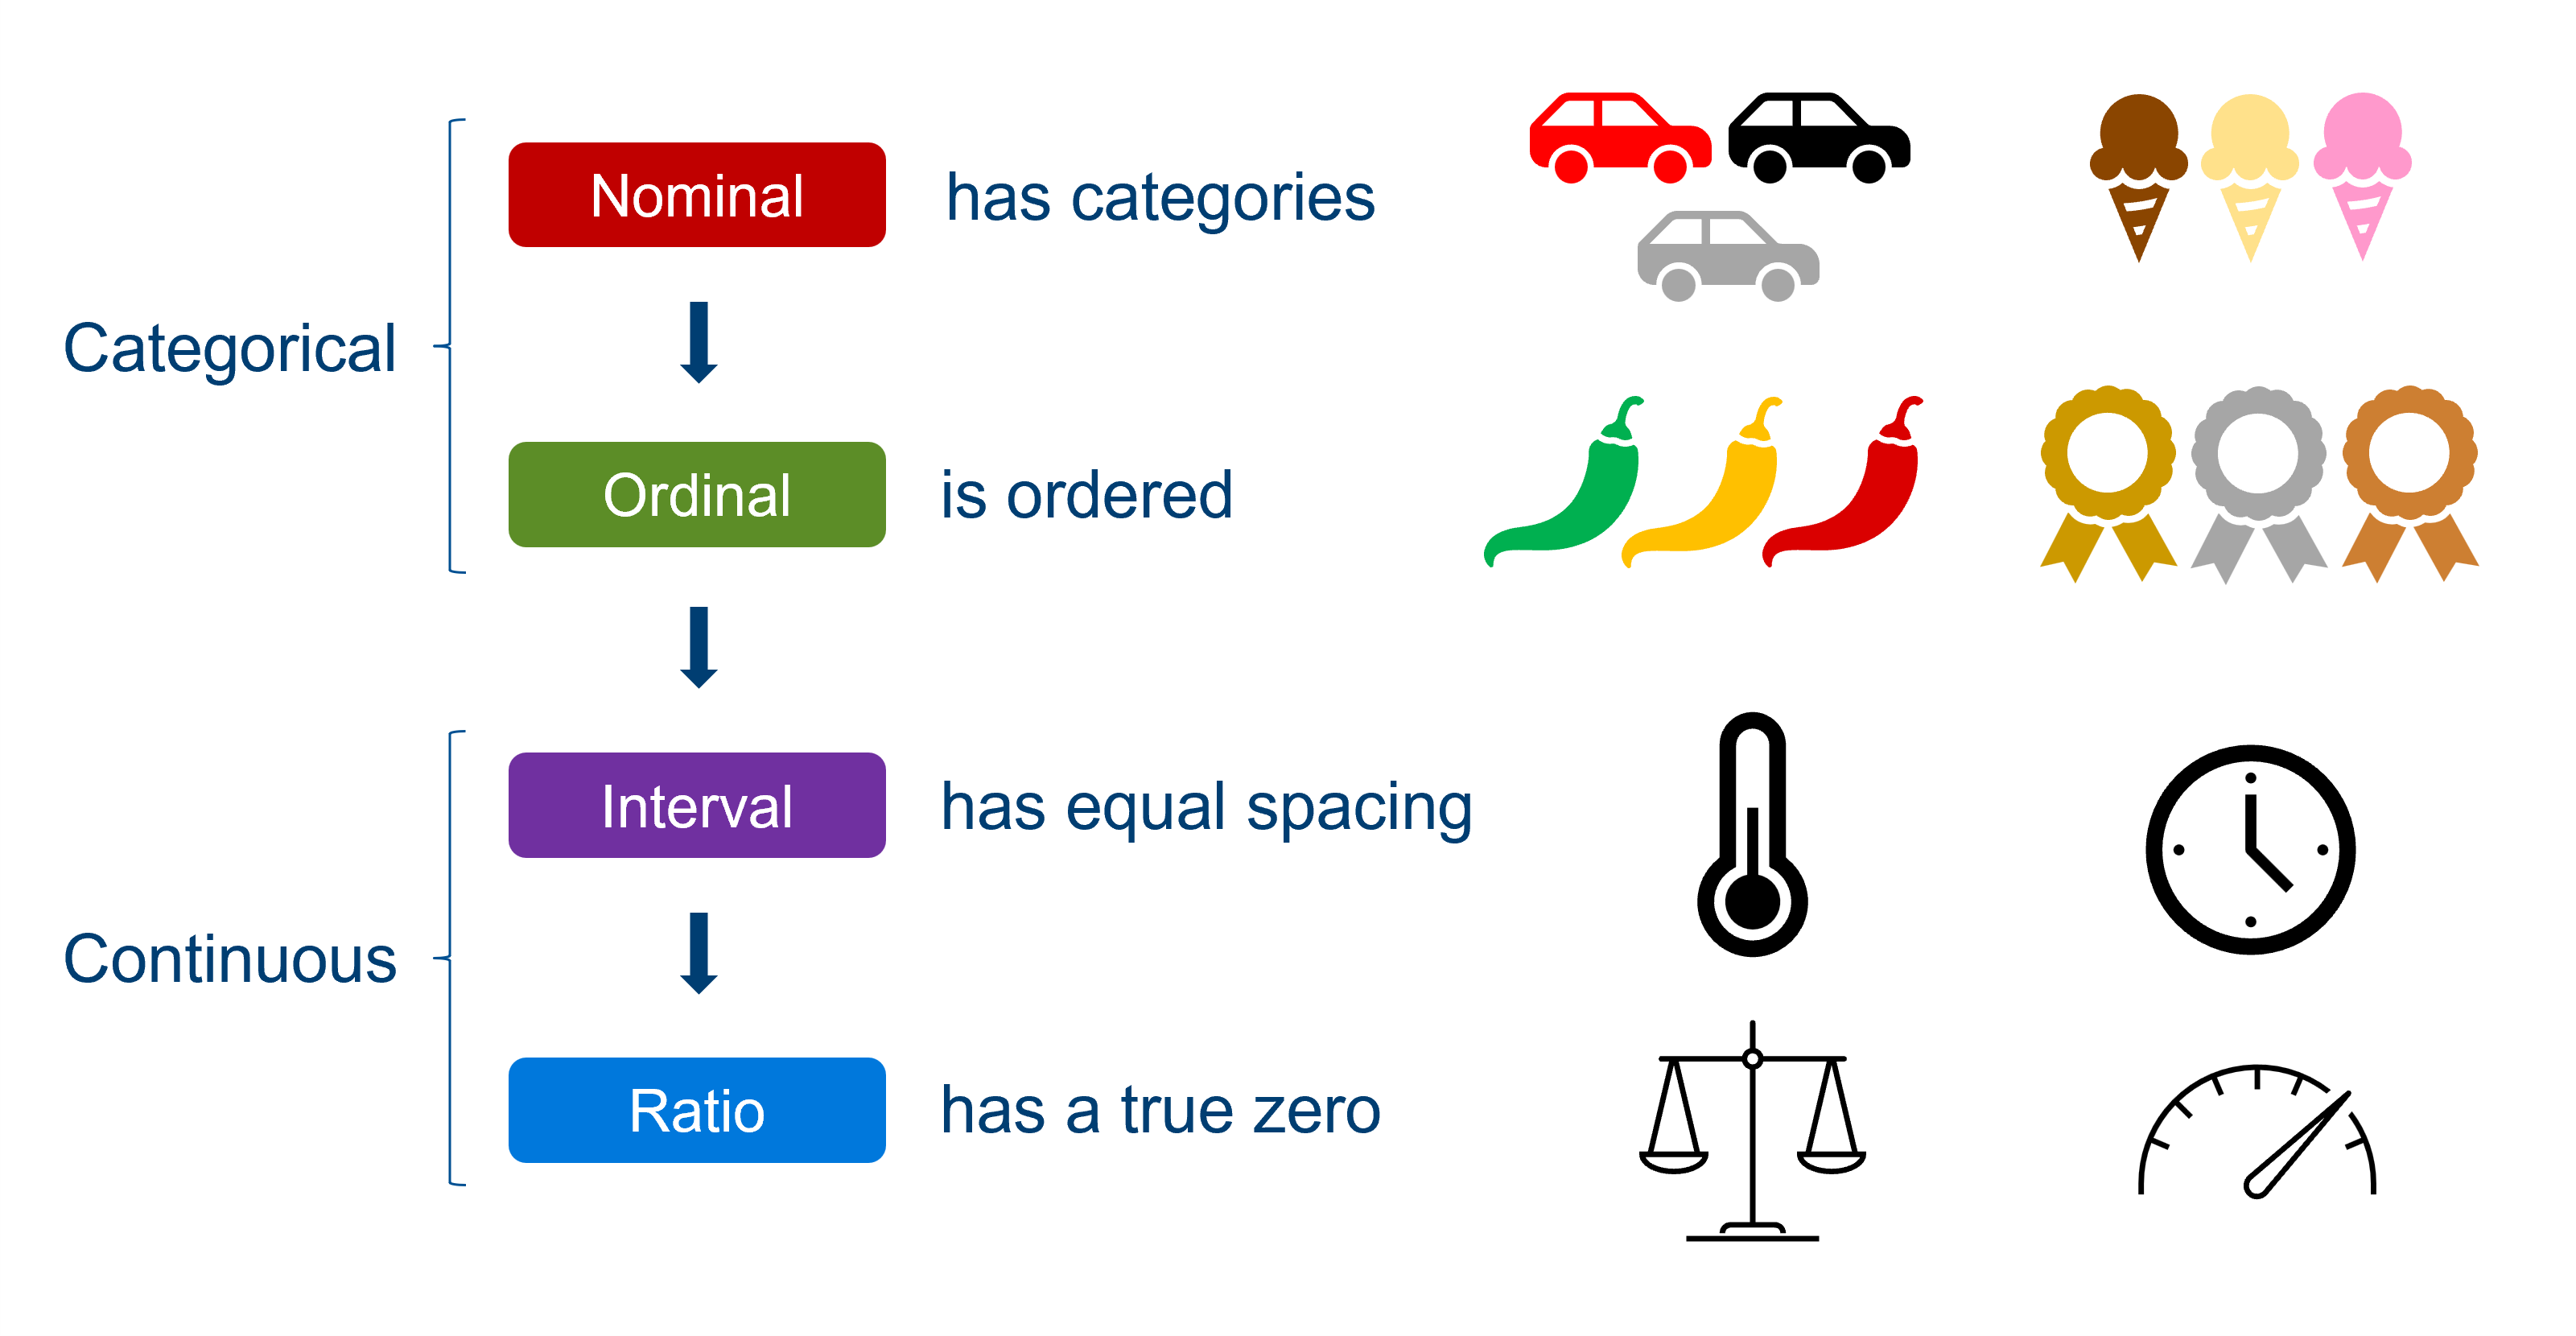
\includegraphics[width=1.1\linewidth]{data-types.png}
    \end{figure}
    
\end{frame}

\begin{frame}{Types of Data Visualization}
\begin{columns}
\column{0.5\linewidth}
     \begin{itemize}
        \item Categorical Variable(s): 
        \begin{itemize}
            \item Bar plot
        \end{itemize}
        \vspace{10pt}
        \item Continuous Variable(s):
        \begin{itemize}
            \item Histogram
            \item Scatter plot
        \end{itemize}
    \end{itemize}
\column{0.5\linewidth}
    \begin{figure}
        \centering
        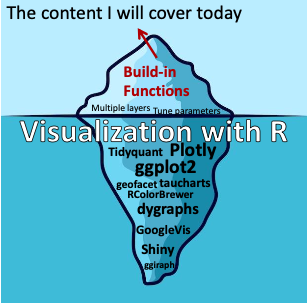
\includegraphics[width=0.95\linewidth]{截圖 2026-03-22 凌晨12.48.55.png}
    \end{figure}
\end{columns}
\end{frame}

\section{Bar Plot}
\begin{frame}[fragile]{Bar Plot}
\begin{itemize}
\item Bar plots are used to compare the frequency of different categories.
\item The height of each bar corresponds to the frequency.
\item \texttt{barplot()}
\end{itemize}


\begin{columns}
\column{0.7\linewidth}
\begin{lstlisting}[basicstyle=\footnotesize\ttfamily]
barplot(data, 
        main = "Title of figure",
        xlab = "Name of X-axis",
        ylab = "Name of Y-axis",
        col = "Color within Bin",
        border = "Color in border of Bin",
        xlim = c(a, b), # Modify range of X-axis
        ylim = c(a, b)  # Modify range of Y-axis
        )
\end{lstlisting}

\column{0.3\linewidth}
\begin{figure}
    \centering
    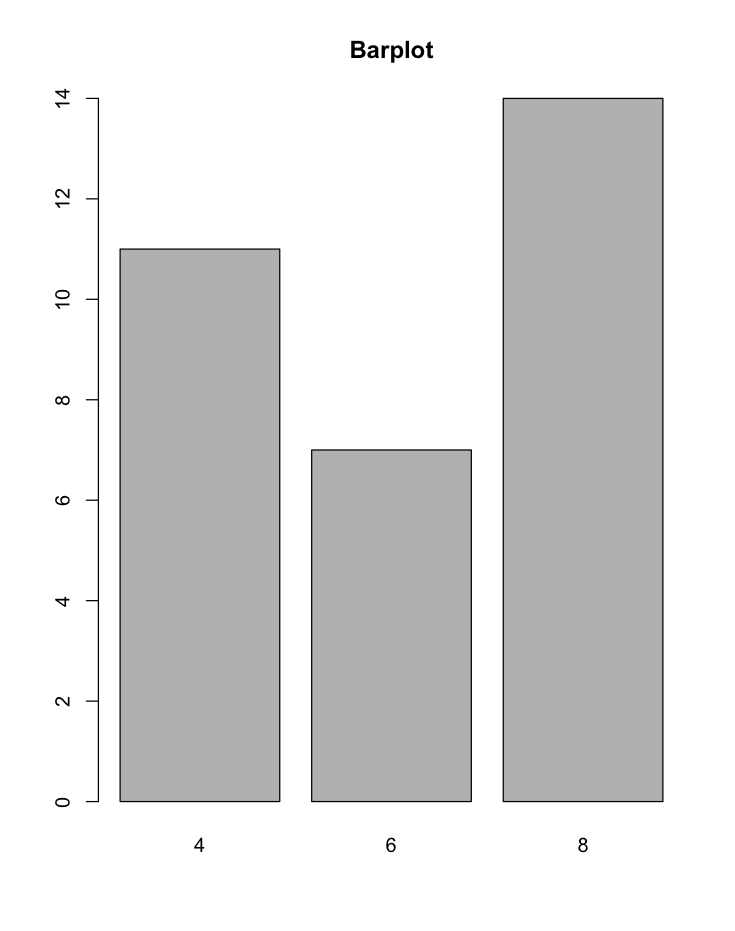
\includegraphics[width=1.25\linewidth]{barplot.png}
\end{figure}

\end{columns}


\end{frame}

\begin{frame}[fragile]{Bar Plot}
We'll use the built-in dataset "penguins" to demonstrate 

\begin{lstlisting}
species <- table(penguins$species)
barplot(species, 
        main = "Numbers of Penguins",
        xlab = "Species",
        ylab = "Counts", 
        col = c("skyblue", "orange", "coral")
\end{lstlisting}
Check \textcolor{blue}{\href{https://r-charts.com/colors/}{Colors in R}} to discover more colors!
\begin{figure}
    \centering
    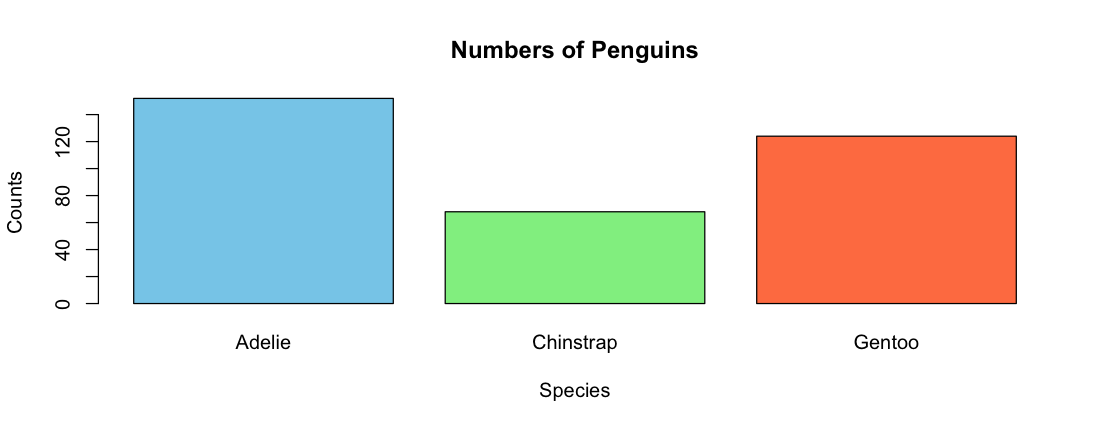
\includegraphics[width=1\linewidth]{penguin_barplot.png}
\end{figure}
\end{frame}

\begin{frame}[fragile]{Multiple Levels Bar Plot}
We'll keep using the "penguins" data to demonstrate 
\begin{lstlisting}[basicstyle=\footnotesize\ttfamily]
species_year <- table(penguins$species, penguins$year)
species_year

barplot(species_year, 
        main = "Numbers of Penguins for Different Year",
        xlab = "Year",
        ylab = "Counts",
        beside = TRUE, 
        legend = TRUE,
        col = c("skyblue", "lightgreen", "coral"))
\end{lstlisting}
\begin{figure}
    \centering
    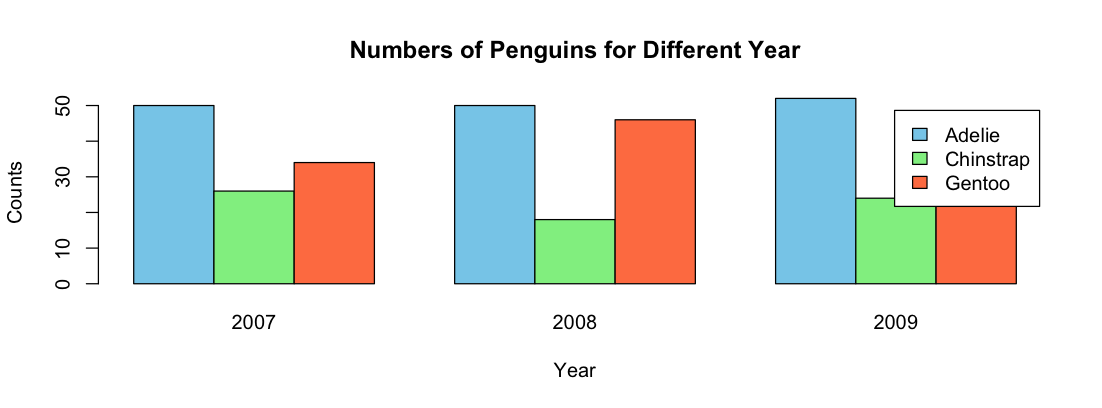
\includegraphics[width=0.95\linewidth]{mutil-level_barplot.png}
\end{figure}
\end{frame}

\section{Histogram}
\begin{frame}[fragile]{Histogram}
\begin{itemize}
    \item Histograms are used to visualize the distribution of continuous variables.
    \item The height of each bin corresponds to the frequency.
\item \texttt{hist()}
\end{itemize}


\begin{columns}
\column{0.7\linewidth}
\begin{lstlisting}[basicstyle=\footnotesize\ttfamily]
hist(data, 
     main = "Title of figure",
     xlab = "Name of X-axis",
     ylab = "Name of Y-axis",
     col = "Color within Bin",
     border = "Color in border of Bin",
     breaks = # Specify how many bins we want
)
\end{lstlisting}

\column{0.3\linewidth}
\begin{figure}
    \centering
    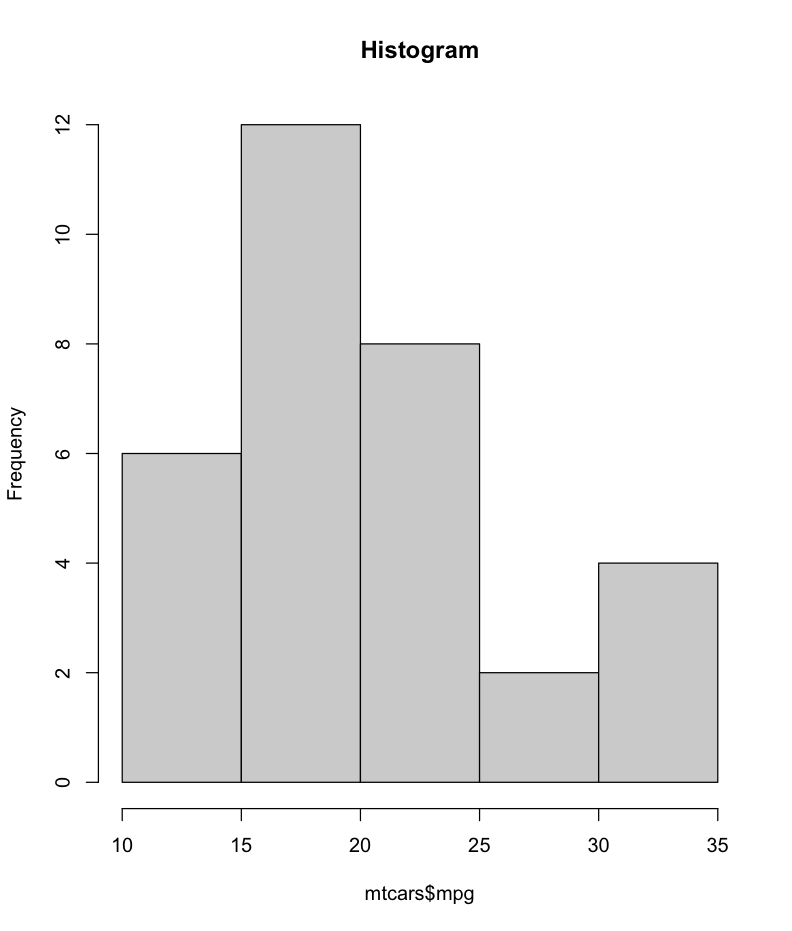
\includegraphics[width=1.25\linewidth]{hist.png}
\end{figure}

\end{columns}
\end{frame}

\begin{frame}[fragile]{Histogram}
We'll use the built-in dataset "trees" to demonstrate 
\begin{columns}
\column{0.7\linewidth}

\begin{lstlisting}
hist(trees$Height,
     main = "Histogram of Tree's Height",
     xlab = "feet (ft)",
     ylab = "counts",
     col = "salmon")

# Use "break" to set the number of bins
hist(trees$Height,
     main = "Histogram of Tree's Height (10 breaks)",
     xlab = "feet (ft)",
     ylab = "counts",
     breaks = 10,
     col = "paleturquoise")
\end{lstlisting}

\column{0.4\linewidth}
\begin{figure}
    \centering
    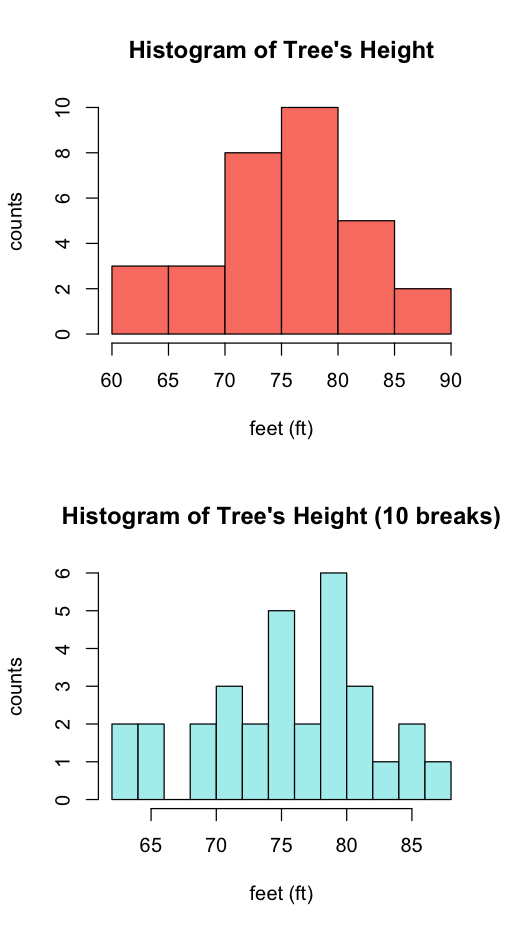
\includegraphics[width=1\linewidth]{histogram.png}
\end{figure}
\end{columns}
    
\end{frame}

\section{Scatter Plot}






\begin{frame}[fragile]{Scatter Plot}
\begin{itemize}
    \item Scatter plots are used to visualize the relationship between two variables.
    \item Each point represents a pair of values.
    \item \texttt{plot()}
\end{itemize}

\begin{columns}[t]
\column{0.7\linewidth}
\begin{lstlisting}[basicstyle=\footnotesize\ttfamily]
plot(data, 
     main = "Title of figure",
     xlab = "Name of X-axis",
     ylab = "Name of Y-axis",
     col = "Color of dot",
     pch = "Shape of dot",
     lty = " Shape of line",
     type = "Type of scatter plot"
)
\end{lstlisting}

\column{0.3\linewidth}
\begin{figure}
    \centering
    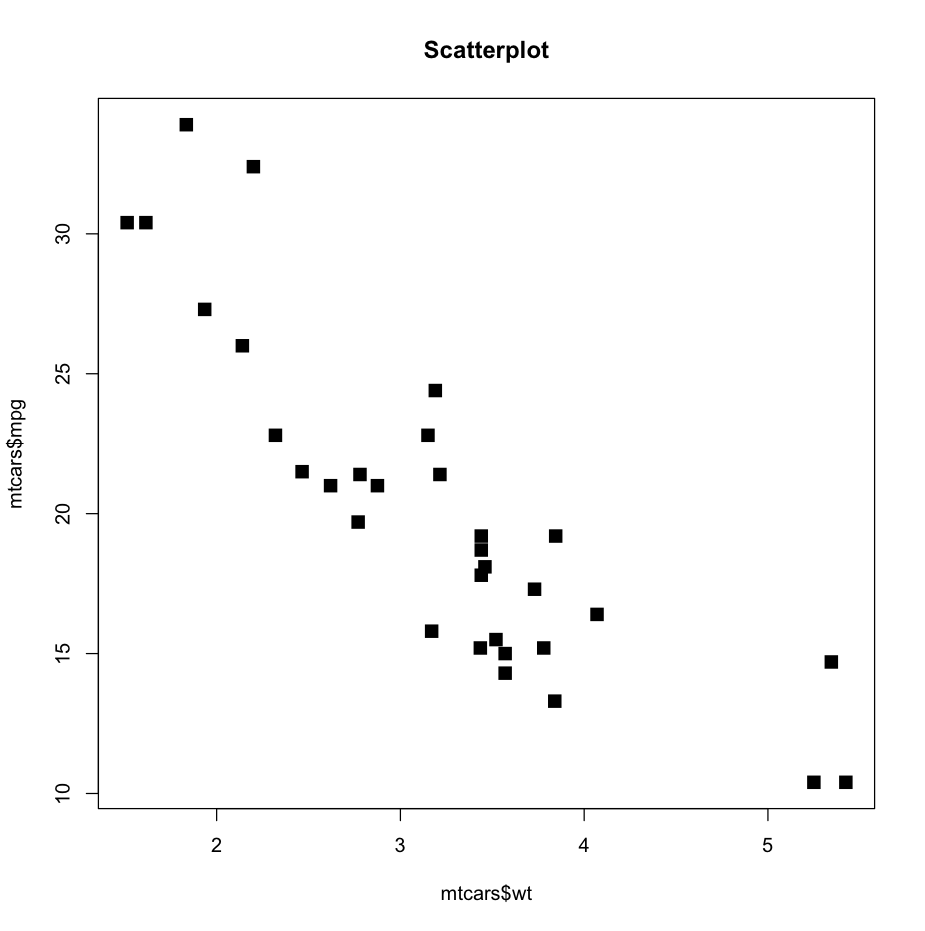
\includegraphics[width=1.1\linewidth]{plot.png}
\end{figure}

\end{columns}


\end{frame}

\begin{frame}[fragile]{Scatter Plot}
We'll use the built-in dataset "women" to demonstrate 
\begin{columns}
\column{0.6\linewidth}

\begin{lstlisting}[basicstyle=\footnotesize\ttfamily]
?women

plot(women)

# Add some settings
plot(women,
     main = "Scatter Plot of Height vs. Weight",
     xlab  = "Inch (in)",
     ylab = "Pound (lbs)",
     pch = 20, 
     col = "brown",
     cex = 3,
     type = "p")
\end{lstlisting}

\column{0.4\linewidth}
\begin{figure}
    \centering
    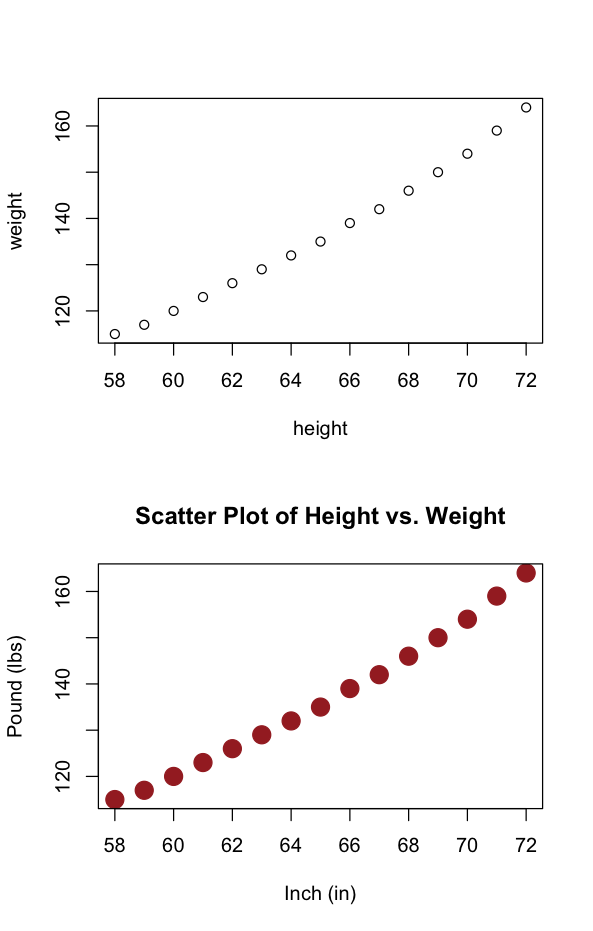
\includegraphics[width=1.1\linewidth]{scplot.png}
\end{figure}
\end{columns}
    
\end{frame}

\begin{frame}{Plot Style}
Check these websites for more plot styles 
\begin{itemize}
    \item Colors (col=): \textcolor{blue}{\url{https://r-charts.com/colors/}}
    \item Plot Symbols (pch=): \textcolor{blue}{\url{https://r-charts.com/base-r/pch-symbols/}}
    \item Line Style(lty=) and Plot Type (type=): \textcolor{blue}{\url{https://r-charts.com/base-r/line-types/}}
\end{itemize}
\end{frame}

\begin{frame}{The End of the Course}
\begin{enumerate}
    \item You don’t need to memorize everything!\\
Google, Stack Overflow, GenAI would be your good friends!
    \item Future exploriation
    \begin{itemize}
        \item Various graph types (\textcolor{blue}{\url{https://r-graph-gallery.com/}})
        \item Plot matrix (combining multiple figures)
        \item tidyverse, ggplot2 (widely used visualization packages)
    \end{itemize}
\end{enumerate}
    
\end{frame}
\section{Lab Report}
\begin{frame}{Lab Report}
\begin{itemize}
    \item The report file will be in the NTU COOL Assignment section
    \item Submit your file in pdf format
    \item Deadline: 3/29 (Sun) 23:59
    \item Late submission is not accepted
\end{itemize}
    
\end{frame}

\end{document}
